\documentclass[11pt,letterpaper]{article}
\usepackage{pdfpages}
\usepackage{fancyhdr}
\usepackage[colorlinks=true, urlcolor=blue, linkcolor=blue]{hyperref}
\usepackage{graphicx}
\usepackage[top=1.4in, left=0.5in, right=0.5in, bottom=0.8in]{geometry}
\usepackage[T1]{fontenc}
\usepackage{helvet}
\pagestyle{fancy}
\renewcommand{\headrulewidth}{0pt}
\renewcommand{\footrulewidth}{0pt}
\setlength{\parindent}{0em}
\setlength{\parskip}{1em}


\fancyfoot[C]{\setlength{\unitlength}{1in}\begin{picture}(5,0)\put(-1.8,-1){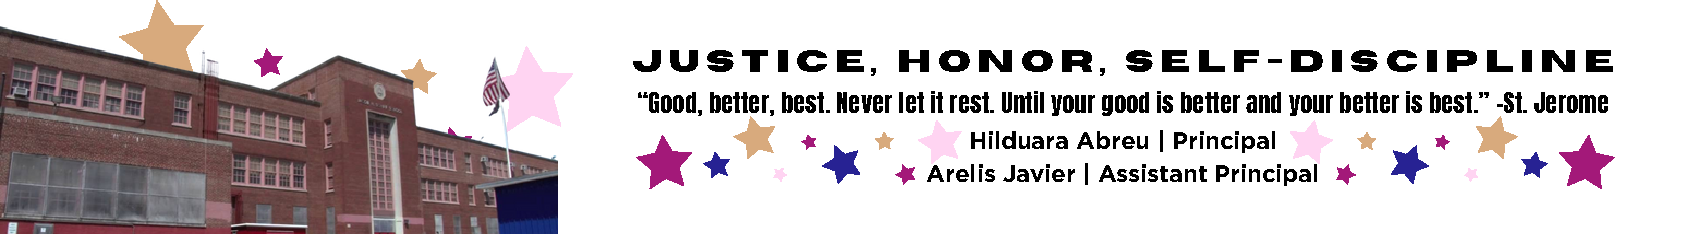
\includegraphics[width=8.8in,height=1.3in]{logo-1}}\end{picture}}
\fancyhead[C]{\setlength{\unitlength}{1in}\begin{picture}(5,0)\put(-1.9,-1){
\includegraphics[width=8.9in,height=1.3in]{logo-2}}\end{picture}}

\pagenumbering{gobble}
\addtolength{\evensidemargin}{-2in}
\addtolength{\topmargin}{-0.5in}
\addtolength{\textwidth}{0in}
%%%%%%%%%%%%%%%%%%%%%%%%%%%%%%%%%%%%%%%%%%%%%%%%%%%%%%%%%%%%%%%%%%

\begin{document}
\vspace*{0.5in}
School Website: \href{https://www.ps192.org/apps/pages/index.jsp?uREC_ID=1504973&type=d&pREC_ID=2359028}{www.ps192.org}

\textbf{Principal's Message December 2023}


Dear Esteemed Families of P.S. 192,

As we embrace the festive cheer of this Holiday Season, I am thrilled to extend our heartfelt wishes to each one of you! It's astounding to reflect on how swiftly the year has progressed; it seems like just yesterday when we welcomed everyone back in September. These past few months have been a whirlwind of vibrant events and enriching educational experiences, each one contributing to the tapestry of memories we've woven together at P.S. 192.

I was particularly delighted to share the joy of Thanksgiving with our wonderful students. The sight of parents and students coming together in celebration was truly heartwarming. Keeping with our cherished tradition, we are excited to once again invite you to our annual Holiday Breakfast. This festive gathering is a perfect occasion for our school community to unite and share in the holiday spirit. Please mark your calendars for this delightful event on Thursday, December 21 at 8:00 a.m., held in our Gym.

I'd also like to remind our dedicated parents that our teachers are available every Tuesday from 2:30 p.m. to 3:35 p.m. post-dismissal. This is an invaluable opportunity to connect with your child’s educators, gain insights into your child's academic journey, and discuss how we can collaboratively foster their growth.

As the holiday break approaches, I encourage our families to dedicate time to engaging in educational activities. Whether it's exploring math problems, enjoying story-time together, or encouraging your children to write and read independently, every moment of learning is precious. I invite you to keep a family journal during the holidays, documenting those special moments and experiences that you'll treasure for years to come.

In closing, on behalf of the entire staff of P.S. 192, I wish you all a safe, joyful, and enriching Holiday Season! May this time be filled with happiness, learning, and cherished memories.

Warmest regards,


\includegraphics[width=0.2\textwidth]{hil_signature}

\textbf{Hilduara Abreu}

\textbf{Principal P.S. 192}

\textit{The School of Joyful Learning!}

\newpage
\vspace*{.5in}
Nuestro Sitio Web: \href{https://www.ps192.org/apps/pages/index.jsp?uREC_ID=1504973&type=d&pREC_ID=2359028}{www.ps192.org}

\textbf{Mensaje de La Directora Para 2023}

Mientras abrazamos la alegría festiva de esta temporada navideña, ¡estoy encantado de extender nuestros más sinceros deseos a cada uno de ustedes! Es sorprendente reflexionar sobre lo rápido que ha avanzado el año; Parece que fue ayer cuando dimos la bienvenida a todos en septiembre. Estos últimos meses han sido un torbellino de eventos vibrantes y experiencias educativas enriquecedoras, cada una de las cuales ha contribuido al tapiz de recuerdos que hemos tejido juntos en P.S. 192.

Me sentí particularmente feliz de compartir la alegría del Día de Acción de Gracias con nuestros maravillosos estudiantes. Ver a padres y estudiantes reunidos para celebrar fue realmente conmovedor. Siguiendo con nuestra querida tradición, nos complace invitarlo una vez más a nuestro desayuno navideño anual. Esta reunión festiva es una ocasión perfecta para que nuestra comunidad escolar se una y comparta el espíritu navideño. Marque en sus calendarios este delicioso evento el jueves 21 de diciembre a las 8:00 a.m., que se llevará a cabo en nuestro Gimnasio.

También me gustaría recordarles a nuestros dedicados padres que nuestros maestros están disponibles todos los martes de 2:30 p.m. a 15:35 post-despido. Esta es una oportunidad invaluable para conectarse con los educadores de su hijo, obtener información sobre el recorrido académico de su hijo y discutir cómo podemos fomentar su crecimiento de manera colaborativa.

A medida que se acercan las vacaciones, aliento a nuestras familias a dedicar tiempo a participar en actividades educativas. Ya sea explorando problemas matemáticos, disfrutando juntos de la hora del cuento o animando a sus hijos a escribir y leer de forma independiente, cada momento de aprendizaje es precioso. Los invito a llevar un diario familiar durante las vacaciones, documentando esos momentos y experiencias especiales que atesorarán en los años venideros.

Para terminar, en nombre de todo el personal de P.S. 192, ¡les deseo a todos unas fiestas seguras, alegres y enriquecedoras! Que este tiempo esté lleno de felicidad, aprendizaje y recuerdos preciados.

El más cálido saludo,


\includegraphics[width=0.2\textwidth]{hil_signature}

\textbf{Hilduara Abreu}

\textbf{Principal P.S. 192}

\textit{The School of Joyful Learning!}
\end{document}
